\chapter{Fundamentação Teórica}

Este capítulo detalha os principais conceitos e tecnologias aplicados no projeto: Internet das Coisas, sistemas distribuídos, protocolo HTTP, AOSP, desenvolvimento Android e ESP32 com NodeMCU. Portanto, 
a seguinte seção aborda como os conceitos citados contribuíram para o desenvolvimento deste trabalho de conclusão de curso, possibilitando
ao leitor uma visão geral das competências necessárias em sua execução. 

\section{Internet das Coisas}

O termo \textit{Internet das Coisas} (\textit{IoT}, da expressão em inglês \textit{Internet of Things}) foi utilizado primeiramente em 1999 pelo então pesquisador do \textit{Massachusetts Institute of Technology} (MIT) Kevin Asthon em uma apresentação na Procter \& Gamble (P\&G) sobre a tecnologia do \textit{Radio Frequency Identification} (RFID). O RFID é uma tecnologia utilizada para a identificação e rastreamento de objetos, animais ou pessoas via ondas de rádio. Portanto, Asthon pontuou a possibilidade de utilizar tal ferramenta para gerenciar a cadeia de suprimentos da empresa, pois sua capacidade de ler vários emissores simultaneamente, sem a necessidade de linha de visão direta entre o leitor e a tag (ao contrário da tecnologia de códigos de barras) torna o monitoramento de cada produto nos distintos pontos de transporte mais fino e mensurável. A ideia do autor 
é que os próprios objetos tenham a capacidade de gerar os dados e reagir aos estímulos do ambiente \cite{iot-first-definition}.

\textit{IoT} possui muitas definições. Embora não haja um consenso convergente para uma definição única, podemos discutir sobre seu impacto na sociedade atual e aspectos importantes que toda solução na área possui. No livro \textit{The Internet  of Things}, escrito por Samuel Greengard, o tema é abordado como um evento disruptivo, onde a linha que separa o humano e a tecnologia se torna cada vez menos visível, porém o texto aborda não somente a capacidade de conexão entre as máquinas, e sim a autonomia e "inteligência" cada vez maior dos sistemas embarcados \cite[pp. 17]{book-iot}. Essa visão de tecnologia integrada no cotidiano é o conceito que o autor Mark Weiser aborda no seu artigo denominadao \textit{The Computer for the 21st Century}. A computação ubíqua é o processo de tornar os computadores ``invisíveis'' aos nossos olhos, desenvolvendo a comunicação com tais ferramentas o mais próximo possível da forma humana, ou seja, o dispositivo tem conexão com a rede e responde aos estímulos do usuário por interfaces naturais, por exemplo, a fala e gestos com as mãos \cite{ubiquitous-computing}.

Portanto, o significado mais comum de \textit{IoT} talvez seja a de dispositivos eletrônicos conectados na internet, permitindo enviar e receber dados do ambiente real. No entanto, apenas conectar dispositivos não é uma solução em Internet das Coisas, pois essa área envolve o uso de protocolos de comunicação, eletrônica de baixo consumo energético, plataformas em nuvens e outras inúmeras áreas do conhecimento. Os dados coletados de sensores atuam como combustível para a execução de um fluxo de tomada de decisão \cite{iot-cycle}. 

\begin{figure}[ht]
    \centering
    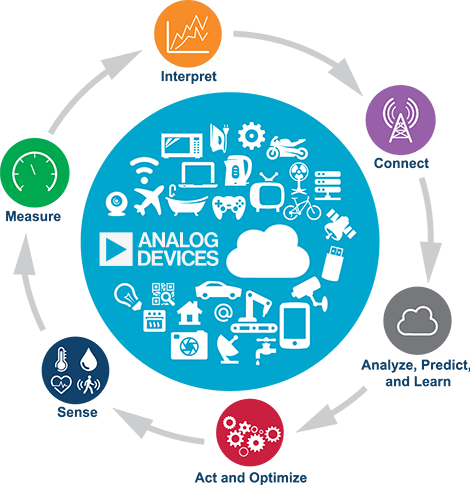
\includegraphics[width=.45\textwidth]{img/iot-cycle.png}
    \caption{Ciclo de IoT. Fonte:\cite{iot-cycle}}\label{figIoTCycle}
\end{figure}

Atualmente, a coleta de dados e uso de ferramentas de análise são o principal recursos de empresas competitivas no gerenciamento de suas atividades. Com o avanço da área de telecomunicações, as organizações têm potencial de transformar grandes volumes de dados em \textit{insights} poderosos, que orientam a tomada de decisões da equipe de gestão. Portanto, a Internet das Coisas representa uma tendência forte e disruptiva na sociedade.

Por exemplo, a Amazon\textsuperscript{\textregistered}, uma das maiores empresas de comércio eletrônico no mundo, anunciou em 2022 o lançamento do robô \textit{Sparrow}, cuja função é manipular objetos em esteiras e realizar o empacotamento
com destreza comparável à de seres humanos. Em suas fábricas, existe um crescente uso de tecnologias de ponta, como robôs autônomos e inteligência artificial, para maximizar as suas entregas em um mercado competitivo \cite{amazon-robos}.

\section{Sistemas Distribuídos}

``Um sistema distribuído é aquele no qual os componentes localizados em computadores interligados em rede se comunicam e coordenam suas ações apenas passando mensagens.'' \cite[pp. 1]{sistemas-distribuidos-coulouris2013}.
A definição apresentada pelo autor leva em conta dois importantes fatores: o primeiro é representado pela comunicação via rede de computadores, e o segundo está relacionado ao provisionamento de um serviço.
O mundo atual oferece inúmeros exemplos da importância dos sistemas distribuídos no desenvolvimento socioeconômico: a modalidade de educação à distância \cite{mec-ead}, no qual serviços web e compartilhamento
multimídia são responsáveis por possibilitar o acesso ao ensino de qualidade ao público distante fisicamente dos grandes centros de ensinos, como, por exemplo, cidades do interior ou comunidades ribeirinhas; o comércio digital, onde a arquitetura do sistema deve suportar picos de acesso em determinados períodos do ano e controle
de concorrência na compra de produtos, deve-se ao crescimento do seguimento de \textit{e-Commerce},
resultou em um faturamento superior à R\$ 180 bilhões de reais em 2023 no Brasil, de acordo com dados da Associação Brasileira de Comércio Eletrônico \cite{abcomm-ecomerce}; e redes \textit{blockchain}, pois as transações distribuídas devem ser auditáveis e transparentes, além do funcionamento descentralizado \cite{juliana-blockchain}, exemplo 
das criptomoedas, pois a tecnologia permite a transferência de recursos e o armazenamento de todas as operações.  

Portanto, o sistema distribuído tem foco no compartilhamento de recursos. Na web, a implementação de arquitetura mais comum é o modelo cliente-servidor, pois
um número grande de aplicações utiliza essa premissa, por exemplo, plataformas de redes sociais, jogos online e serviços bancários.
Ao nível do Sistema Operacional, a comunicação entre processos executados em diferentes computadores interligados em rede é essencial para o gerenciamento e acesso aos recursos distribuídos.
Nesse contexto, um cliente, que pode ser um processo ou aplicativo, realiza uma solicitação ao servidor para acessar ou manipular um recurso, como arquivos, impressoras, ou mesmo capacidade de processamento. O servidor, 
ao receber essa solicitação, desencadeia uma série de operações internas, que podem incluir desde a autenticação do cliente até a busca de dados em um banco de dados distribuído. Em seguida, o servidor 
retorna o resultado ao cliente em espera, completando o ciclo de comunicação do tipo requisição e resposta \cite[pp. 16]{sistemas-distribuidos-coulouris2013}.

\section{HTTP: Fundamentos e Impacto na Web}

O HTTP (do inglês \textit{HyperText Transfer Protocol}) é o protocolo pertencente à camada de aplicação
responsável por definir a estrutura de mensagens HTTP e a forma do programa cliente e do programa servidor 
trocarem suas mensagens individuais. Seu funcionamento obedece à arquitetura cliente-servidor, ou seja, o
usuário (geralmente um navegador Web) envia uma requisição ao servidor, que deverá processá-la e responder 
com um resultado, denominado resposta. O exemplo descrito é o uso de navegadores para requisitar uma página web, porém 
o protocolo HTTP é extensível, pois a comunicação descrita se aplica ao acesso dos mais variados tipos de recursos, graças a
um conceito denominado URL (Uniform Resource Locator), responsável por identificar de maneira única um objeto na internet \cite[pp. 72]{redes-kurose2010}.

\subsection{Padrão de mensagem HTTP}

No protocolo, existem dois tipos de mensagem: requisição e resposta. Na mensagem de requisição, temos o elemento
chamado \textbf{método}, esse campo define qual a ação que o usuário deseja executar, sendo comum o uso de verbos
como GET, POST, HEAD, PUT e DELETE. Por exemplo, ao realizar o preeenchimento de um formulário de cadastro do site, o
navegador web realiza uma requisição do tipo POST ao servidor, pois sua intenção é a criação de um recurso,
neste caso, a nova conta. A ação é executada sobre um \textbf{caminho}, que corresponde à organização interna dos recursos 
dentro do servidor, por exemplo, as informações sobre produtos estão no caminho ``/product''. O \textbf{cabeçalho} contém informações como: preferência de linguagem,
credenciais de acesso, tipo de conteúdo na mensagem, entre outros. Por fim, o último campo é o \textbf{corpo da mensagem}, 
onde ficam armazenados os dados \cite[pp. 77]{redes-kurose2010}.

\begin{figure}[ht]
    \centering
    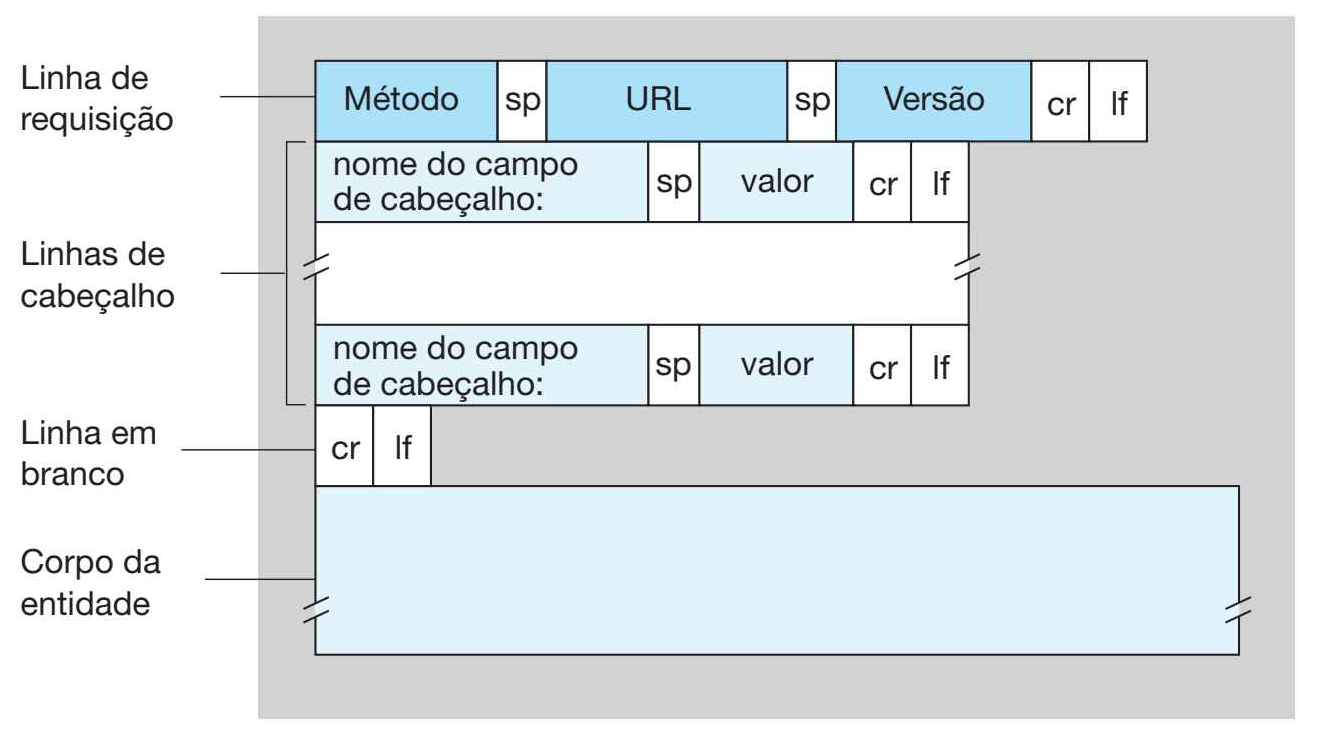
\includegraphics[width=.55\textwidth]{img/mensagem-http-solicitação.png}
    \caption{Padrão de mensagem de solicitação HTTP. Fonte:\cite{redes-kurose2010}}\label{figMessageRequest}
\end{figure}

A mensagem de resposta é constituída de 3 componentes principais: linha de estado, linha de cabeçalho e corpo de entidade. Na \textbf{linha de estado}, um campo
interessante é o \textit{status code}, número pré-definido que indica se o resultado da requisição foi bem-sucedido, ou não, assim como o motivo. No \textbf{cabeçalho}
são adicionadas pelo servidor informações como o tipo do objeto e seu tamanho em bytes. Por último, o \textbf{corpo da mensagem} em si, contendo os dados solicitados \cite[pp. 78]{redes-kurose2010}.

\begin{figure}[ht]
    \centering
    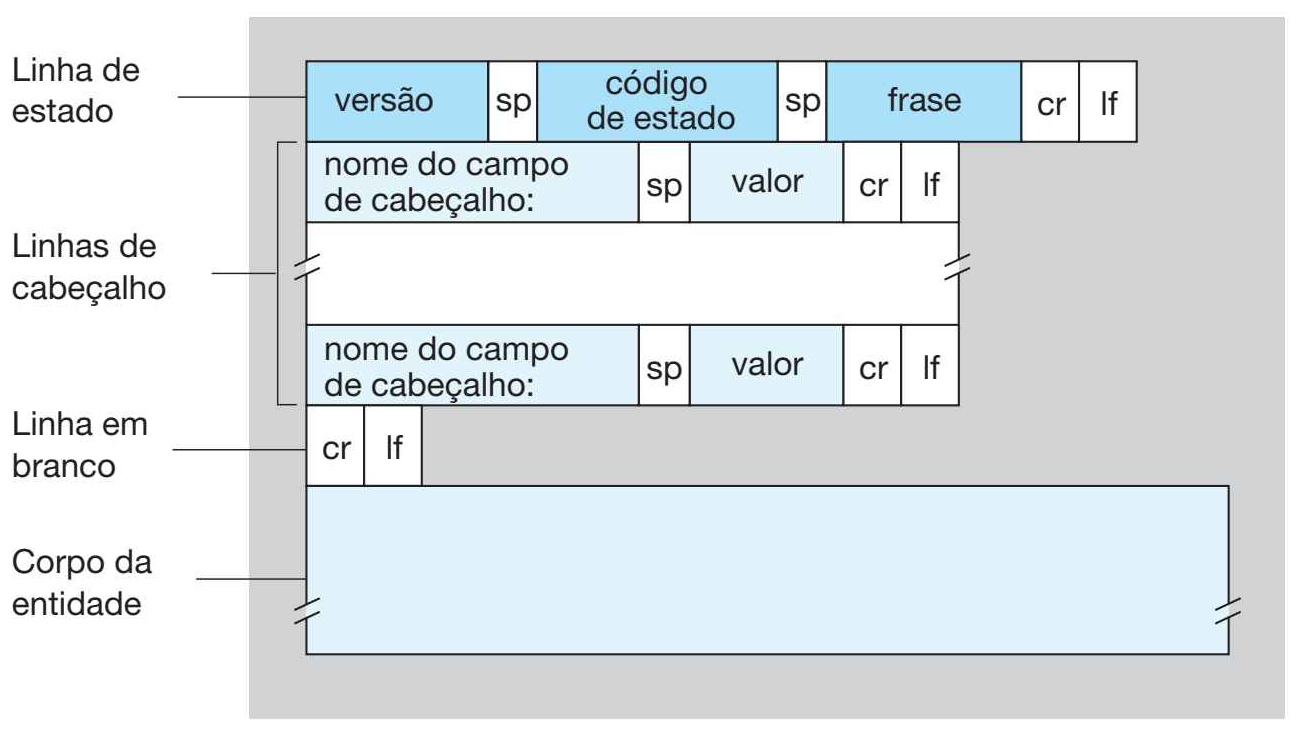
\includegraphics[width=.55\textwidth]{img/mensagem-http-resposta.png}
    \caption{Padrão de mensagem de resposta HTTP. Fonte:\cite{redes-kurose2010}}\label{figMessageResponse}
\end{figure}

\subsection{API}

API é o acrônimo de \textit{Application programming interface}, cuja função é estabelecer um conjunto de padrões e funções
para que diferentes sistemas de software possam se comunicar, executar ações e trocar dados \cite{api-definition}. Por exemplo, a biblioteca
\textit{OpenGL} foi construída como uma API de computação gráfica, responsável por renderizar e modelar objetos no espaço tridimensional independente
de dispositivos de \textit{hardware} \cite{opengl-example}. Outra API bastante utilizada é a \textit{Google Maps API}, pois é um serviço da empresa Google\textsuperscript{\textregistered} 
para acessar dados de geolocalização muito utilizado em sites de hotéis, divulgação de lojas e uso pessoal para encontrar lugares \cite{google-maps-example}. Portanto, API é um recurso 
prático, pois é transparente ao desenvolvedor de software, porém, sem a necessidade de conhecer os procedimentos internos.

O padrão REST (Representational State Transfer) é um estilo de arquitetura de sistemas web 
que provê acesso uniforme aos recursos de um servidor, por meio de uma interface coerente que aplica uma mudança de
estado através das operações básicas do protocolo HTTP, com importância maior aos dados do que a operação e baixo acoplamento entre sistemas. 
Além disso, essa interface de comunicação de sistemas via HTTP garante que cada recurso seja acessível por
uma URL e a interação da API, seja \textit{stateless}, ou seja, a requisição contém toda a informação necessária
para sua execução pelo servidor \cite[pp. 384--386]{sistemas-distribuidos-coulouris2013}. 

Portanto, o desenvolvimento de uma API no padrão REST é útil para a integração entre diferentes sistemas e  padronização das mensagens 
utilizando o protocolo HTTP. As principais vantagens na escolha do REST são: interoperabilidade, onde o 
dispositivo eletrônico envia os dados obtidos e o aplicativo Android consome os eventos, realizando a 
gestão da conta do usuário, com todas essas operações na API comunicadas de maneira uniforme; independência 
de estado, já que o dispositivo pode perder a conexão, mas ao restabelecê-la, deve garantir a comunicação correta; e simplicidade 
na evolução do sistema, uma vez que o modelo suporta comunicação com múltiplos clientes.

\begin{figure}[ht]
    \centering
    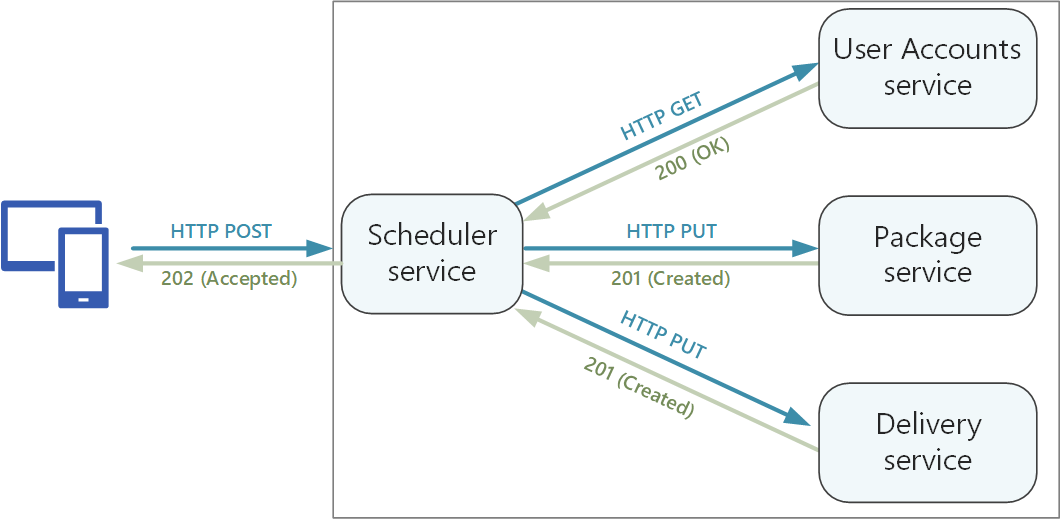
\includegraphics[width=.45\textwidth]{img/api-design.png}
    \caption{Example de design de API para microsserviços. Fonte:\cite{example-design-api}}\label{figAPIDesign}
\end{figure}

\section{AOSP}

O Android é um Sistema Operacional de código aberto com foco em dispositivos móveis, como, por exemplo, \textit{smartphones} e \textit{tables}, baseado na kernel do Linux. 
Liderado pela empresa Google\textsuperscript{\textregistered}, o \textit{Android Open Source Project} (AOSP) é o projeto de código aberto que provê o código-fonte 
do Android e todas as ferramentas necessárias para a construção de personalizações na plataforma, assim como têm o papel de garantir compatibilidade entre as 
versões do projeto e centralizar as contribuições de desenvolvedores do mundo inteiro \cite{aosp-documentation}. O AOSP utiliza uma arquitetura multicamada
na comunicação com o \textit{hardware}, pois o design modular permite flexibilidade, escalabilidade e facilidade de manutenção para que o seu uso em diferentes dispositivos tenha o foco
em otimização no uso de recursos. 

A seguir, será detalhada a estrutura interna do AOSP, destacando o funcionamento de suas camadas e como elas se interligam para otimizar o desempenho e a
compatibilidade com diferentes dispositivos. Essa análise vai explorar como a arquitetura multicamada do AOSP facilita a personalização, a manutenção e o
desenvolvimento contínuo do sistema operacional Android, assim como discutir a colaboração entre desenvolvedores para garantir sua evolução.

\begin{figure}[ht]
    \centering
    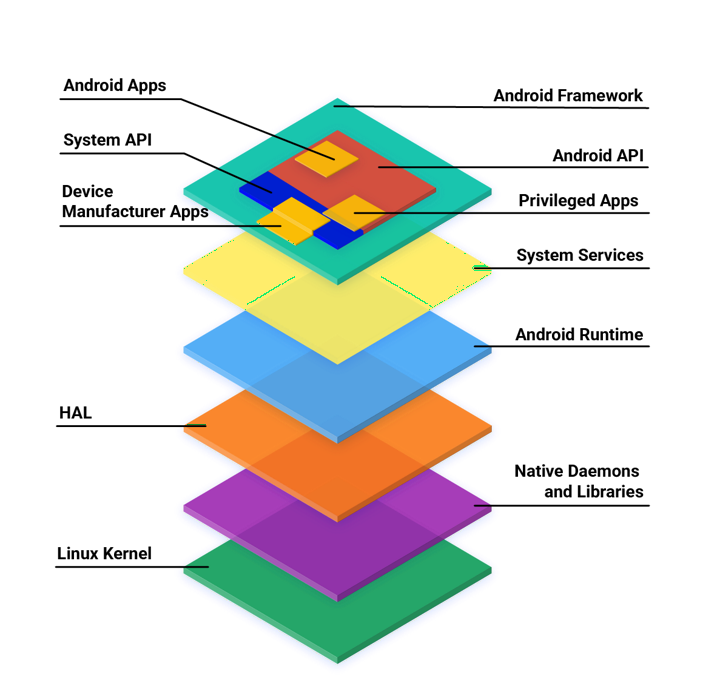
\includegraphics[width=.55\textwidth]{img/android_stack_720.png}
    \caption{Arquitetura do AOSP. Fonte:\cite{aosp-documentation}}\label{figArchAOSP}
\end{figure}

A camada de nível mais alto em abstração é a de \textit{Framework}. Sua função é atuar como porta de entrada para o Sistema Operacional, assim como
estabelecer a comunicação do usuário, por meio de aplicativos ou interação com a interface do Android, com o dispositivo físico por \textit{API} (Application Programming Interface).
Portanto, essa camada provê serviços e funções para desenvolvedores de \textit{software}, por exemplo, manipular a câmera, lanterna ou solicitar acesso à internet. Logo abaixo, existe 
a camada \textit{System Services}, responsável por gerenciar componentes modulares com foco específico. Um exemplo é o \textit{Window Manager}, pois seu papel é gerenciar as janelas e o modo de exibição na tela, 
enquanto o \textit{Media Server} oferece interfaces padronizadas para a utilização de multimídia, como a câmera e áudio.

O \textit{Android Runtime} é o atual ambiente de execução (máquina virtual Java) usado pelo Android, substituindo o antigo \textit{Dalvik}. 
Portanto, todos os aplicativos são executados nessa camada e compilados em \textit{bytecode} para execução na máquina virtual. Em seguida,
o próximo nível é a HAL (\textit{Hardware Abstraction Layer}), a camada de abstração de hardware disponibiliza a definição 
de uma interface e padrão de acesso para os componentes de hardware, pois os desenvolvedores da camada de \textit{Framework} podem acessar 
esses dispositivos de maneira simplificada, sem preocupação com detalhes de implementação, \textit{drivers} e bibliotecas específicas de cada fabricante. A 
\textit{Native Daemons and Libraries} é a camada que expõe funcionalidades de bibliotecas nativas escritas em C/C++ para aplicativos via camada de \textit{Framework} \cite{google-developers-architecture}. 
Essa possibilidade é útil na manipulação de funções de baixo nível e desenvolvimento de extensões para a plataforma, por exemplo, em dispositivos mais específicos, como uma 
máquina de pagamento, que necessita do uso de um sistema de impressão.

Ao final, o \textit{Linux Kernel} representa o Sistema Operacional, de fato, em sua pura essência. É interessante destacar que o Android utiliza 
uma versão do Linux com algumas adições especiais, como o \textit{low memory killer}, que é um sistema de gerenciamento de memória mais agressivo, pois trabalha com recursos 
limitados e tem a premissa de que memória livre é memória com desperdício . Diante disso, o \textit{kernel} trabalha com os apps em segundo plano, permitindo que o usuário navegue 
entre diferentes aplicações sem afetar significativamente o desempenho do seu aparelho \cite{google-developers-memory-killer}. Outro exemplo é o sistema de \textit{wake locks}, que é um serviço de energia que evita 
a drenagem da bateria em situações de ociosidade \cite{google-developers-wakelock}.

\section{Desenvolvimento de aplicativos Android}

O Android possui uma extensa documentação, fornecendo os fundamentos para o desenvolvimento de 
aplicativos de alta qualidade e resilientes. Portanto, essa seção abordará as melhores práticas e recomendações
de arquitetura para a construção de aplicativos com uma experiência de usuário fluida e consistente. Tais práticas envolvem o profundo
conhecimento de componentes de aplicativo, fluxos de trabalho e ciclo de vida da camada de visualização. Ao seguir uma arquitetura, 
o desenvolvedor de \textit{software} consegue melhorar sua produtividade e a qualidade de entregas, pois uma base de código aderente ao 
padrão escolhido facilita a manutenção, desenvolvimento de novas funcionalidades e promove a colaboração entre equipes \cite{google-developers-guideline}.

\subsection{Recomendação de Arquitetura}

Um princípio muito usado na área de desenvolvimento de software é o chamado \textit{separation of concerns}, ou separação de responsabilidades. Esse conceito, no ecossistema Android,
atua na divisão do sistema em partes menores, específicas para uma determinada função e com um objetivo bem definido. Por exemplo, não misturar lógica de 
negócio ou acesso aos dados na camada de visualização (UI), tornando-a  responsável apenas pela interação com o usuário. Diante disso, a documentação recomenda a separação em (pelo menos)
duas camadas principais: \textit{UI} e \textit{Data}. A camada de \textit{UI} é responsável por exibir os dados do aplicativo, refletindo a mudança na tela em resposta às
interações do usuário (como cliques ou pressionamento de botões) ou a eventos externos (como a resposta de uma requisição de rede). Por sua vez, a camada \textit{Data} fornece à camada de \textit{UI} 
um acesso simplificado aos dados, além de abrigar a lógica de negócio e o gerenciamento adequado de cada tipo de dado. Opcionamente, pode-se adicionar uma terceira camada entre as duas chamada de \textit{Domain Layer}.
Sua função é intermediar a comunicação entre as duas camadas, abstraindo chamadas e eventos em um lugar centralizado \cite{google-developers-guideline}.

\begin{figure}[ht]
    \centering
    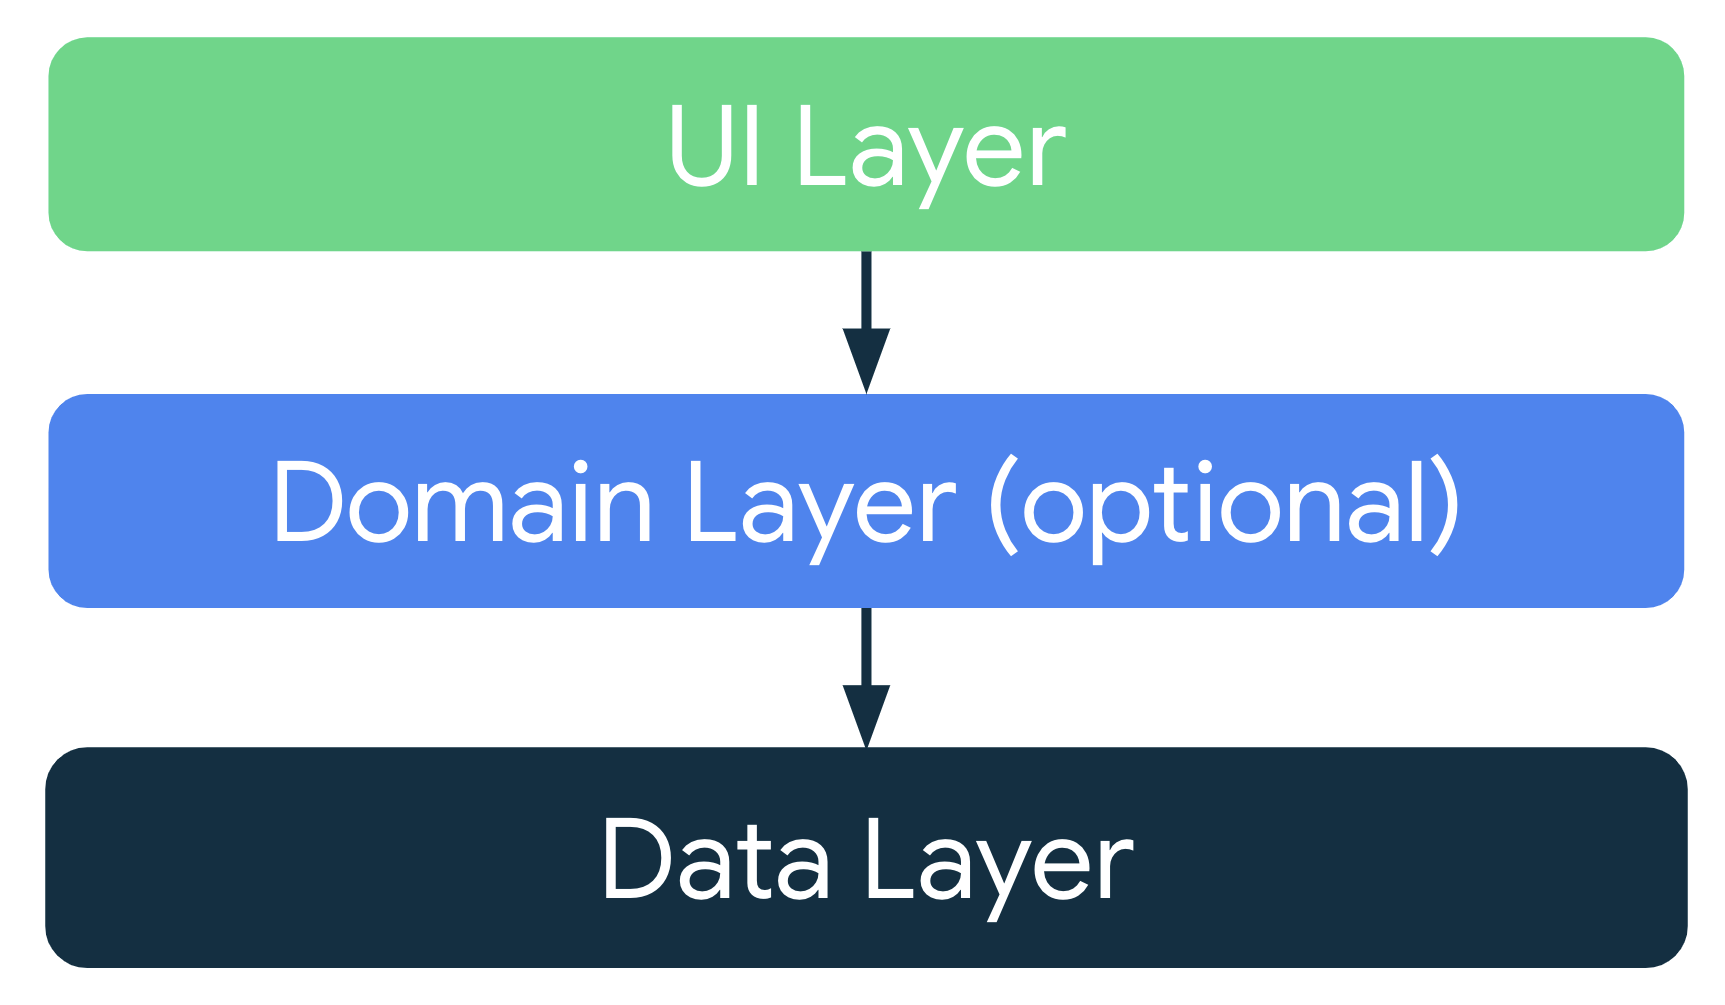
\includegraphics[width=.73\textwidth]{img/app-android-layers.png}
    \caption{Camadas de arquitetura (App). Fonte:\cite{google-developers-guideline}}\label{figAppLayer}
\end{figure}

\subsection{Ciclo de vida da atividade}

O \textit{Activity lifecycle} (ciclo de vida de uma atividade) descreve todos os estados pelos quais uma activity passa, do momento em que é criada
até quando é destruída. Uma \textit{activity} é uma classe que fornece uma janela para o aplicativo desenhar sua interface de usuário, pois um projeto Android 
inicia sempre com uma \textit{activity}. O ciclo de vida de uma \textit{activity} passa por cinco etapas: 
\textit{initialized}, \textit{created}, \textit{started}, \textit{resumed}, \textit{destroyed}. A seguir, será explicado o que ocorre em cada 
uma delas e suas especificidades.

\begin{figure}[ht]
    \centering
    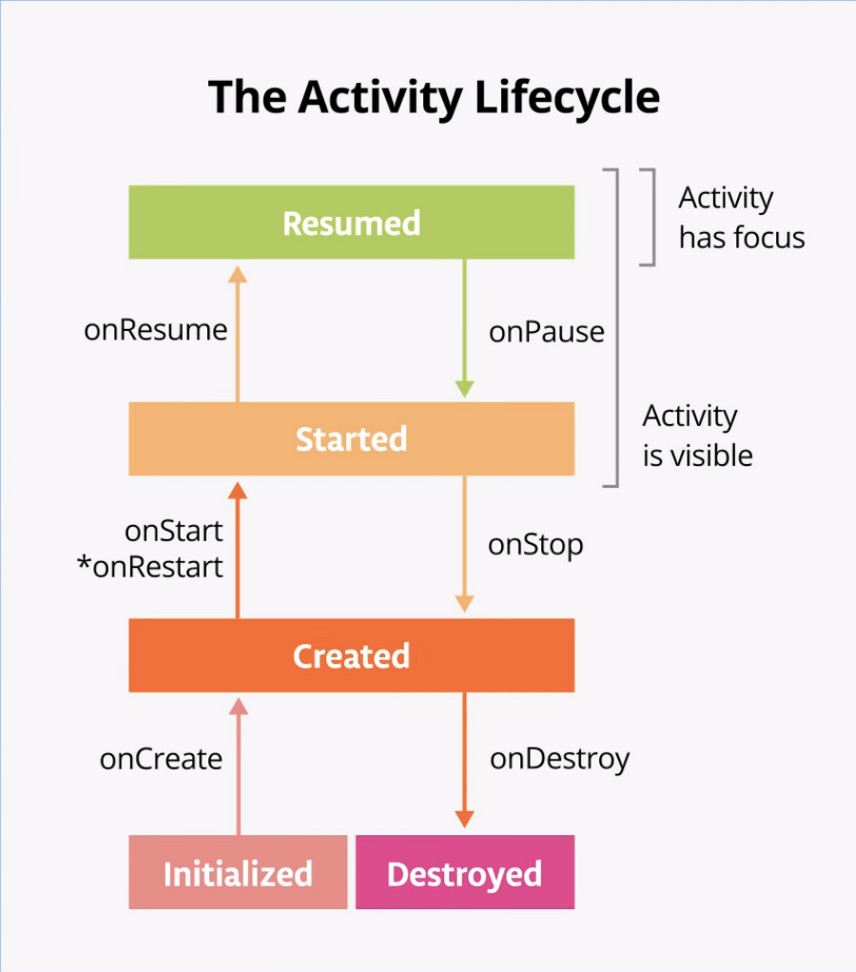
\includegraphics[width=.37\textwidth]{img/activity-lifecycle.png}
    \caption{Ciclo de vida de uma \textit{activity}. Fonte:\cite{google-developers-activity-lifecycle}}\label{figActivityLifeCycle}
\end{figure}

Quando a \textit{activity} é criada pelo sistema, o estado \textit{created} é ativado. Nesse estágio, os recursos da interface gráfica 
são inicializados, porém, a janela ainda não está disponível ao usuário. A partir do estado \textit{started}, os componentes da \textit{activity} são exibidos e a tela se torna visível, porém sem interação.
O estado \textit{resumed} é o aplicativo em primeiro plano, recebendo interações com o usuário em pleno exercício de suas funções. No entanto, se o usuário realizar uma ação que tire 
o foco do aplicativo (como verificar um e-mail após receber uma notificação), a \textit{activity} entrará no estado de pausa (paused).
Caso o usuário volte ao aplicativo, a \textit{activity} retoma os estados \textit{started} e \textit{resumed}, restaurando a interação. No entanto, se o usuário não retornar e a \textit{activity} for fechada, 
ela passará para o estado \textit{destroyed}, encerrando seu ciclo de vida.

\subsection{Arquitetura MVVM}

\section{ESP32}